
\begin{figure}[t]
  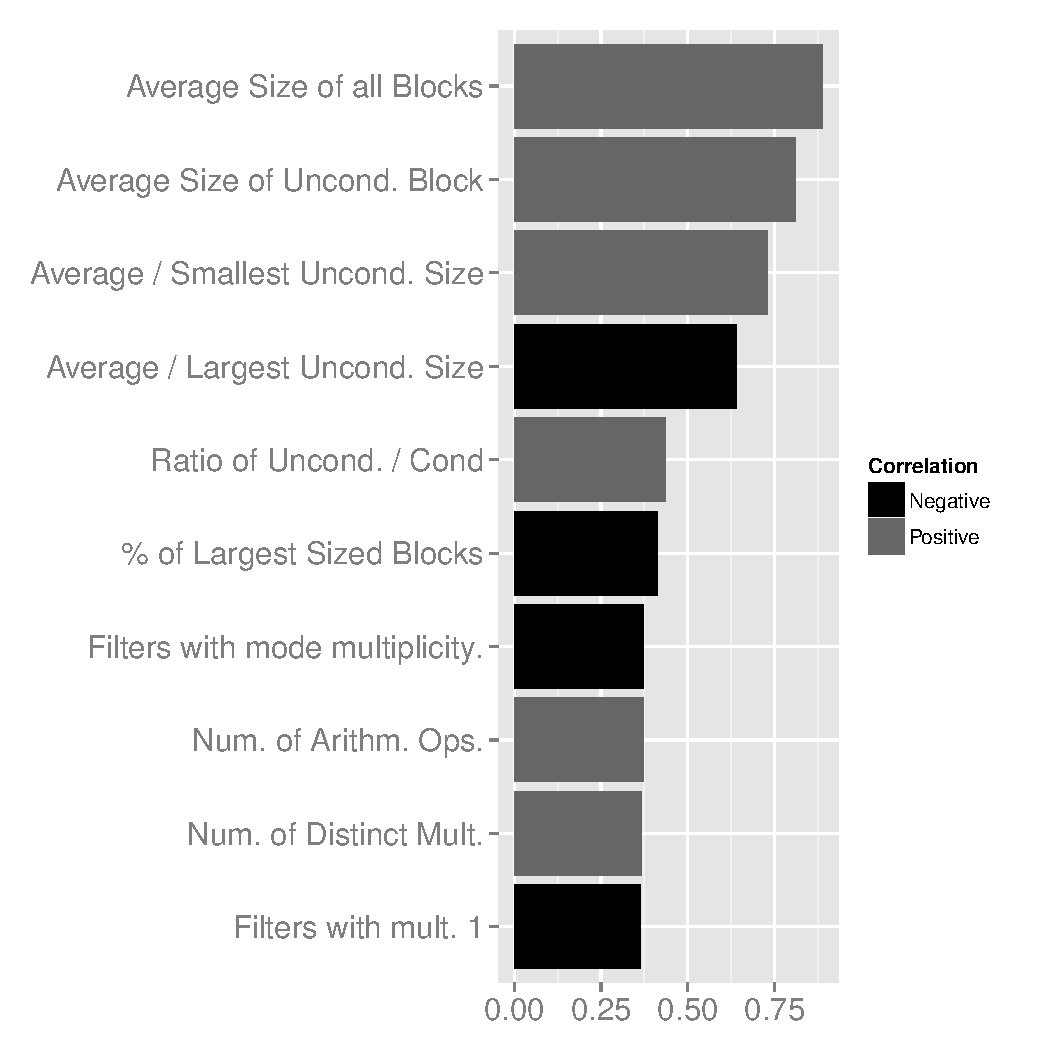
\includegraphics[width=1\textwidth]{streamit-paper/graphics/coreCorr.pdf}
  \caption{The ten highest correlating features with the optimal number of cores.}\label{fig:corrCore}
\end{figure}

\begin{figure}[t]
  \center
  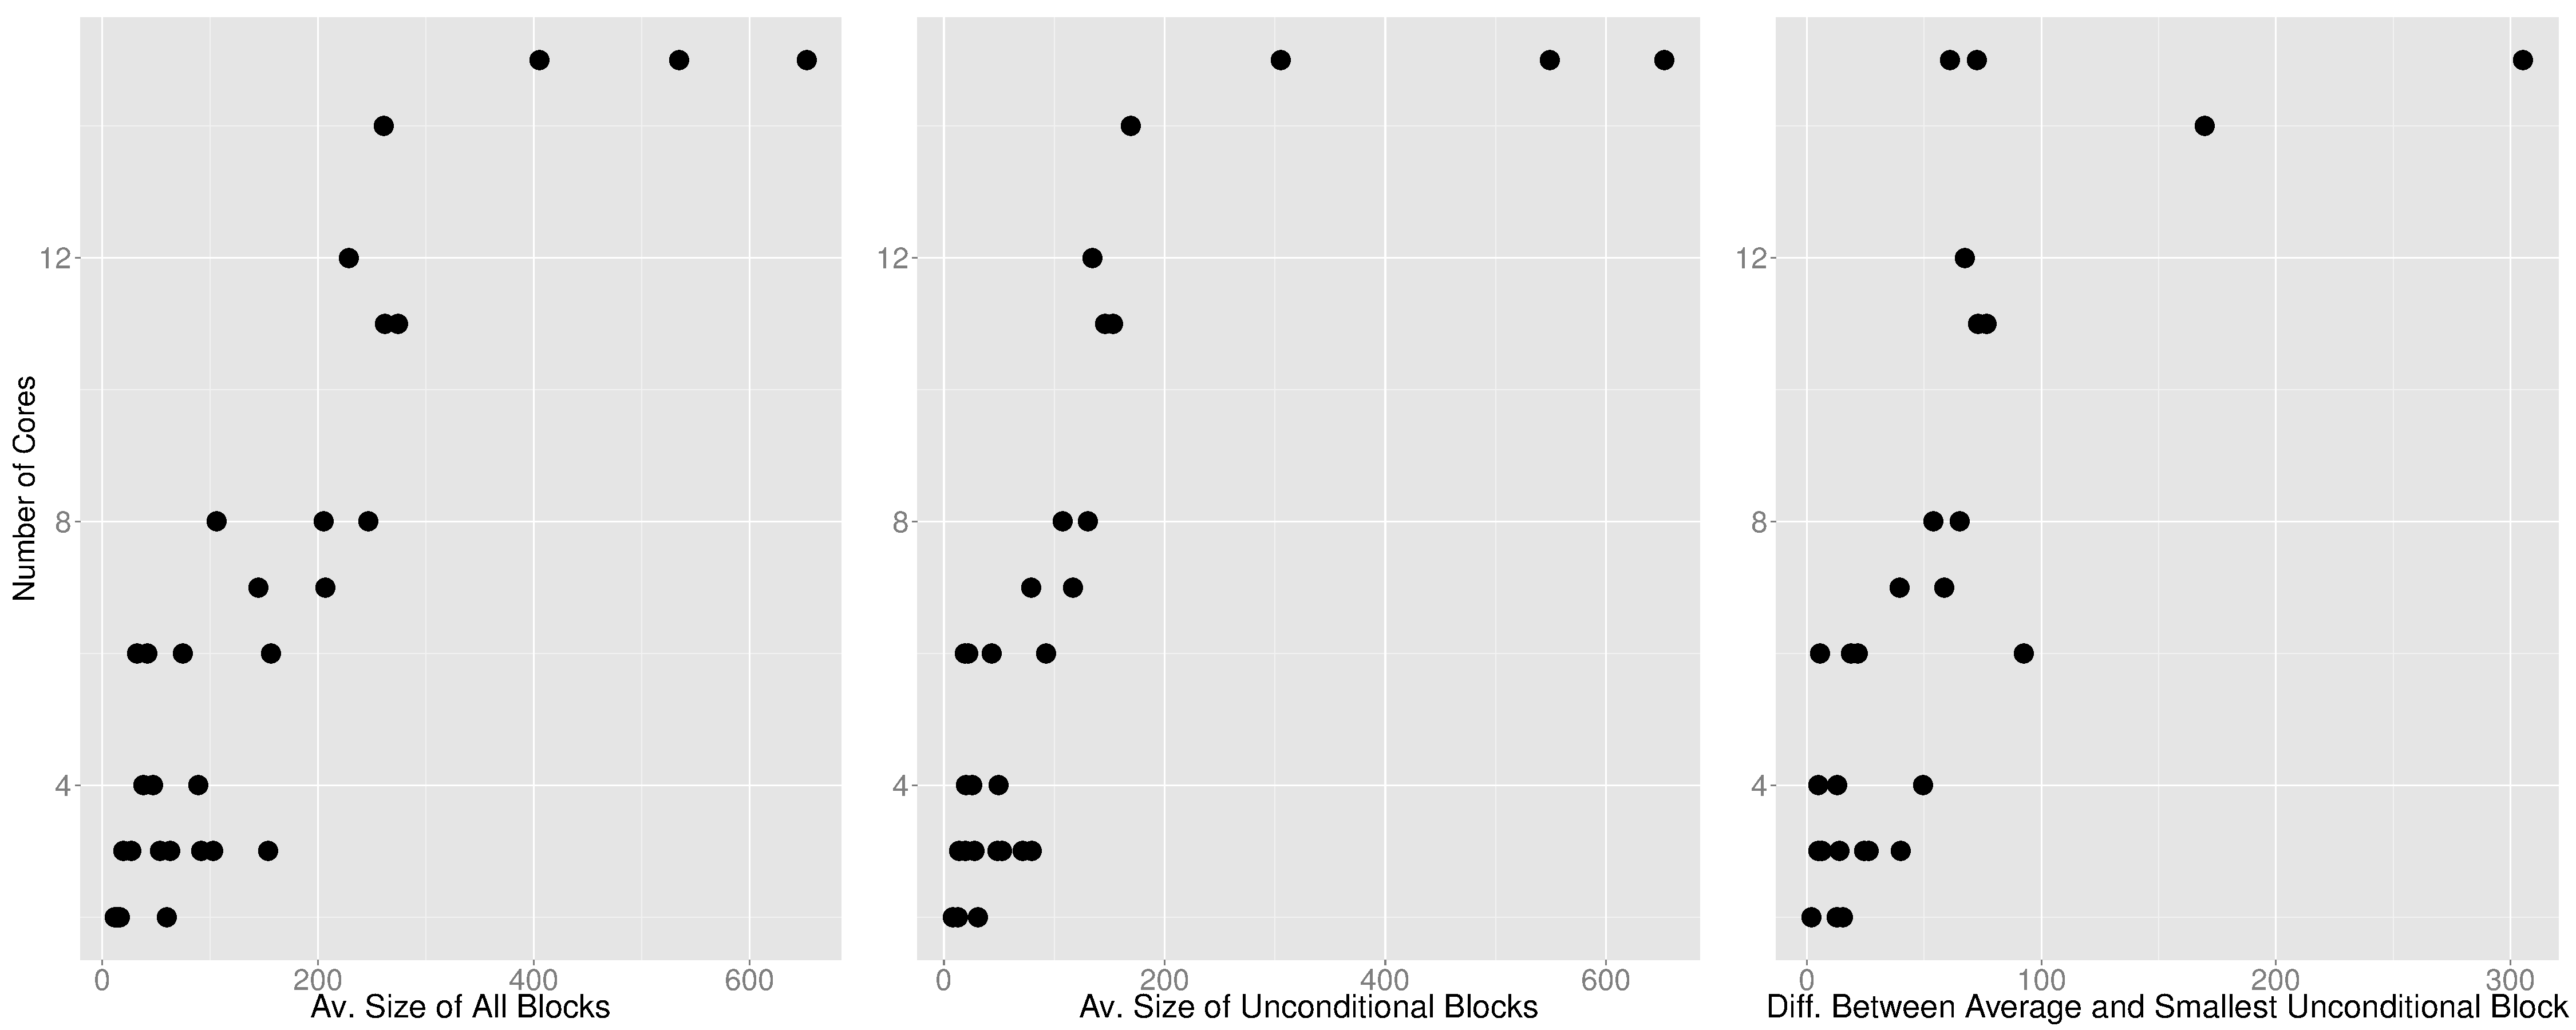
\includegraphics[width=1\textwidth]{streamit-paper/graphics/lineargraphs.pdf}
  \caption{Optimal number of cores in relation to the three highest correlating features. The maximum number of cores plateaus on the right hand side as this is the maximum possible amount.}\label{fig:maxav}
\end{figure}


\subsection{Gathering Training Data}
Given that the optimal number of cores for a thread is independent of the number of threads found in the program, only the single threaded versions is used to determine the optimal number of cores.
For example, all benchmarks will only have a single core per thread when the application is partitioned in 15 threads as this is the maximum amount of cores that may be given to each thread rather than it being the optimal solution. 
Multiple versions of the benchmarks using different amounts of unrolling are included.
To determine the optimal number of cores only the training data that has a performance within 1\% of the best is selected. 

\subsection{Analyzing Features}

Figure~\ref{fig:corrCore} shows the highest correlating features with the optimal number of cores.
The features are very different from the ones presented in Figure~\ref{fig:corr} and overall there are higher correlating features.
The highest correlating value has a correlation factor of 0.88 which represents the number of operations found in a basic block of code.
The second feature is similar but only takes into account blocks that will be executed unconditionally, we have chosen to exclude blocks found in loops for this metric as there is still some form of condition for those blocks to be executed.
The next two feature compare the size of the average size of an unconditional block to the largest and smallest unconditional block.
The fifth feature measures the ratio of the number of unconditional blocks to conditional.

Overall there are no features distinct to StreamIt, such as pipelines or splitjoins that correlate highly with the optimal number of cores.
This is due to the fact that, from a single-threaded perspective, splitJoins and pipelines are less visible in terms of performance.
This is especially true of splitjoins as they will not be distributing data amongst different threads and, technically, a single-threaded StreamIt program is a long pipeline structure.
It can thus be infered that the optimal number of cores is independent of the structure of a StreamIt program.
Instead, it is more dependent on the amount of computation found in each program.

From Figure~\ref{fig:corrCore} the highest correlating features fit naturally under the assumptions that higher core compositions will perform better with larger blocks.
This is due to the fact that large blocks reduce the amount of branches predicted to populate all the cores with blocks which, in turn, reduces the latency of fetching blocks for all cores.
The necessity to correctly predict blocks to ensure that all cores are fully utilised explains why a higher number of unconditionally executed blocks compared to conditional blocks correlates highly.
This is once again due to reducing strain on branch prediction for higher core compositions.
StreamIt programs tend to not have a large quantity of conditional statements, thus the ratio of unconditional and conditional blocks is considered less important than the sizes of blocks.

Other features that were analysed included more fine-grained data on what types of operations were found in the blocks of code.
This involved finding ratios of floating point, integer and memory operations.
According to the correlation graph in Figure~\ref{fig:corrCore}, the composition of these blocks of code are not as important as their size or whether they are conditionally executed.

%Added text for thesis
%EDGE architecture's ability to fetch atomic instruction blocks and out-of-order execution encourages the focus on determining how much speculation is extracted from each filter.
%Unfortunately StreamIt programs do not tend to have a large quantity of conditional statements and when they do they tend to be quite small.
%This statement is reinforced by the correlation between the average number of conditional blocks with the optimal number of cores, which is only 0.2, compared to 0.809 for the average size of unconditional blocks.
%Thus there is no focus on using any speculative features from the StreamIt graph.

\subsection{Linear Regression Model}
Given that the optimal number of cores is highly correlated with a few features, a linear regressor is a natural choice to predict the best number of threads.
Figures~\ref{fig:maxav} represent how the first three highest correlating values affect the number of cores.
This figure was obtained by finding the best number of cores for a single threaded benchmark.
It is important to note that the top right corner points will always be flat as we can only allocate a maximum of 15 cores.

